%% Final Project report — Wireless Networks (EE702020)
%% Based on bare_jrnl.tex (IEEEtran V1.4b, Michael Shell), one-column journal mode.
%% Compile with pdfLaTeX on Overleaf; figures are in ./figures, references in references.bib.

\documentclass[journal,onecolumn]{IEEEtran}

\usepackage{cite}
\usepackage{amsmath,amssymb}
\usepackage{graphicx}
\graphicspath{{figures/}}
\usepackage{array}
\usepackage{multirow}
\usepackage[caption=false,font=footnotesize]{subfig}
\usepackage{url}
\usepackage{algorithm}
\usepackage{algpseudocode}
\usepackage{tikz}
\usetikzlibrary{positioning,arrows.meta,shapes.geometric,fit,calc}

\hyphenation{op-tical net-works semi-conduc-tor}

\begin{document}

\title{Reducing the Labeling Overhead of Learning-Based mmWave Beam Selection via Active Learning}

\author{Nguyen Phuong Lam (Student ID: XXXXXXXX), Duong Minh Hieu (Student ID: XXXXXXXX)
  \thanks{Final Project report, Wireless Networks (EE702020), Faculty of Electrical and Electronics Engineering, Ton Duc Thang University, 2026.}% <-this % stops a space
\thanks{Instructor: Assoc. Prof. Duc Ngoc Minh Dang }}

\markboth{Wireless Networks (EE702020) Final Project, 2026}%
{Reducing the Labeling Overhead of mmWave Beam Selection via Active Learning}

\maketitle

\begin{abstract}
  Sensing-aided beam selection, which predicts the best millimeter-wave (mmWave) beam from camera or LiDAR data, is a promising way to reduce the beam-training overhead of vehicular 5G and 6G links. However, training such a predictor requires many samples labeled by exhaustive beam sweeps. Existing active learning (AL) methods reduce this labeling cost but keep only the index of the best beam, discarding the power measured for every other beam and treating all prediction errors as equally costly. We propose Power-Aware Active Learning (PAAL), which reuses this power profile, at no extra measurement cost, to train on soft labels, score unlabeled samples by their expected power loss in dB, and select diverse batches with a loss-weighted k-center rule. We evaluate PAAL against five AL baselines on two real-world 60~GHz datasets, FLASH and DeepSense~6G, with camera and LiDAR modalities, labeling budgets of 5--50\% of the pool, and three runs per setting. Soft labels alone improve every method in all four dataset--modality settings, by up to 12.9 points of top-1 AUC on FLASH. PAAL outperforms all baselines in three of the four settings. On FLASH, it reaches 60\% top-1 accuracy with 50\% fewer labeled samples than random sampling; on DeepSense, it reaches the target accuracy with 15--20\% of the pool, whereas random sampling does not reach it within 50\%. Its selection step adds less than 4~ms per round over Core-set. These results show that exploiting the full beam-sweep power profile effectively reduces the labeling overhead of learning-based mmWave beam selection.
\end{abstract}

\begin{IEEEkeywords}
  Active Learning, mmWave Beam Selection, Labeling Overhead, Soft Labels, LiDAR, FLASH, DeepSense 6G.
\end{IEEEkeywords}

\IEEEpeerreviewmaketitle

%% ======================================================================
\section{Introduction}\label{sec:intro}

Millimeter-wave (mmWave) links support high data rates, but signal loss and blockage make communication difficult. Narrow beams help maintain a link, so the transmitter and receiver must select a beam pair before data can be sent~\cite{heath2016overview}. Standards such as IEEE 802.11ad and 5G NR use beam training for this task. The devices test beams from a codebook and choose the pair with the highest received power~\cite{giordani2019tutorial}. The search takes longer as the codebook grows, and it must be repeated when a vehicle moves or an obstacle blocks the signal. Camera images, LiDAR point clouds, and GPS data can help a model predict a suitable beam without testing every beam~\cite{klautau2019lidar,charan2022vision,salehi2022flash,alkhateeb2023deepsense}. On FLASH, a predictor that uses sensor data reduced beam selection time by 57\% compared with an exhaustive search~\cite{salehi2022flash}. However, training such a predictor still requires labeled data. Each label is the best beam measured by an exhaustive sweep at a given location. These sweeps remain a major cost before deployment, and data must be collected again for each new site, device, or codebook. AL can lower this cost by asking an oracle to label only selected samples. It starts with a small labeled set, ranks the remaining samples, labels the most useful ones, and retrains the model~\cite{settles2009survey,ren2021survey}.

A prior study applied deep AL to wireless communications and found that GALAXY~\cite{zhang2022galaxy} reached the same accuracy on FLASH with up to 50\% fewer labels than standard training~\cite{soltani2024learning}. Still, most AL methods keep only the index of the strongest beam. An exhaustive sweep also measures the received power of every beam, and this information is important because prediction errors have different costs. A beam near the strongest one may lose less than 1~dB, while a distant beam may lose tens of dB. Several beams may have similar power, and some beams occur much more often than others. Thus, one class label does not show the quality of the other beams, and it treats all errors as equally costly. Existing work also does not clearly separate the effect of richer training labels from the effect of the query strategy. We address these gaps with PAAL. It uses the measured power profile to form soft training labels, estimate the expected power loss of each unlabeled sample, and select a diverse batch with a weighted k-center rule. We evaluate PAAL offline on FLASH~\cite{salehi2022flash} and DeepSense~6G~\cite{alkhateeb2023deepsense}, using camera and LiDAR modalities. We compare five AL baselines with hard and soft labels, test query strategies under the same soft-label setting, and run ablation tests. We follow the protocol in~\cite{soltani2024learning}, but limit the labeling budget to 5\%--50\% of each training pool.

The main contributions of this work are as follows:
\begin{itemize}
  \item We propose PAAL, which reuses the power profile in three components. It trains the predictor on soft labels derived from the measured powers, scores each unlabeled sample by its expected power loss using a power-loss matrix estimated from the labeled sweeps, and selects diverse batches with a k-center rule weighted by this loss. PAAL needs no measurements beyond the usual sweep and adds less than 4~ms per selection round over Core-set.
  \item We compare PAAL with five representative AL baselines on two real-world 60~GHz datasets that differ in codebook size, sensor placement and power coverage. FLASH uses 34 sectors and measures only part of them in each sweep, whereas DeepSense~6G uses 64 beams and measures all of them. Both camera and LiDAR modalities are evaluated. Each baseline is trained with both hard and soft labels, which separates the effect of the training target from that of the query strategy, and an ablation study isolates the contribution of each PAAL component.
  \item We show that soft labels from the power profile improve every method in all four dataset--modality settings, by up to 12.9 points of top-1 AUC, without extra sweeps. With soft labels for all methods, PAAL outperforms every baseline in three of the four settings and reaches 60\% top-1 accuracy on FLASH with 50\% fewer labeled samples than random sampling. We also report the settings in which PAAL does not win and discuss possible reasons, to guide the choice of query strategy for each modality.
\end{itemize}

The rest of the paper is organized as follows. Section~\ref{sec:lit} reviews related work. Section~\ref{sec:method} defines the problem and presents PAAL. Section~\ref{sec:eval} describes the datasets, baselines, implementation details, evaluation protocol, and results. Section~\ref{sec:conclusion} gives the main findings, limitations, and future work.

%% ======================================================================
\section{Literature Review}
\label{sec:lit}

\subsection{Sensing-Aided Beam Selection}
In 802.11ad and 5G NR, beam management relies on sweeping a codebook of beams during initial access and repeating the sweep to track the beam as the user moves~\cite{giordani2019tutorial}. The time spent on these sweeps grows with the number of beams, and narrow mmWave beams are easily misaligned by mobility and blockage, so the overhead is especially high in vehicular links~\cite{heath2016overview,giordani2019tutorial}. This has motivated the use of out-of-band side information, i.e., data from sensors that observe the environment, to predict the best beam and shorten or skip the sweep.

Klautau \emph{et al.}\ used LiDAR for this purpose: a deep network trained on LiDAR occupancy data from ray-traced vehicular scenes selects a short list of candidate beams, so that only these beams need to be swept~\cite{klautau2019lidar}. Their study showed that LiDAR captures the obstacles that determine the propagation paths, but it relied on simulated data. Charan \emph{et al.}\ moved to real measurements and fused camera images with GPS positions to predict the beam on DeepSense~6G~\cite{charan2022vision}. DeepSense~6G is a large-scale real-world dataset that records camera, LiDAR, radar and GPS data together with the received power of all beams of a 64-beam phased array across many scenarios~\cite{alkhateeb2023deepsense}, which provides a common benchmark for sensing-aided beam prediction on real data. Salehi \emph{et al.}\ released FLASH, a 60~GHz vehicular dataset collected with commercial IEEE 802.11ad radios together with GPS, camera and LiDAR data, and proposed a multimodal fusion network trained with federated learning; their predictor reduced the beam selection time by 57\% compared with an exhaustive search~\cite{salehi2022flash}.

These studies show that sensor data can replace most of the beam sweep at run time, and that combining modalities usually improves accuracy. However, all of them train the predictor in a fully supervised way on large labeled datasets, where every label comes from an exhaustive sweep. The cost of collecting these labels is not addressed, although it must be paid again whenever the predictor is deployed at a new site or with a different codebook.

\subsection{Deep Active Learning}
Active learning reduces labeling cost by letting the learner choose the samples to be labeled~\cite{settles2009survey}. In the pool-based setting considered here, a large set of unlabeled samples is available, and the learner repeatedly selects a batch, queries an oracle for its labels, and retrains~\cite{settles2009survey,ren2021survey}. For deep networks, this setting raises specific difficulties: models must be retrained in every round, batches must be selected at once rather than one sample at a time, and the initial model is trained on very few labels~\cite{ren2021survey}.

Uncertainty-based methods select the samples on which the current model is least certain. Classical criteria include least confidence, the margin between the two most likely classes~\cite{scheffer2001active}, and the entropy of the predicted distribution~\cite{settles2009survey}. Gal \emph{et al.}\ estimated model uncertainty in deep networks with Monte Carlo dropout and selected samples with high disagreement between stochastic forward passes~\cite{gal2017deep}. Uncertainty criteria are simple and cheap, but in batch mode they tend to select many similar samples, and they depend on the calibration of the network.

Diversity-based methods instead select samples that represent the whole pool. Sener and Savarese formulated batch selection as a core-set problem and solved it with a greedy k-center algorithm on the network embeddings, which selects samples far from those already labeled~\cite{sener2018coreset}. This avoids redundant batches but ignores how informative each sample is. Hybrid methods combine the two ideas. BADGE runs k-means++ seeding on gradient embeddings, whose magnitude reflects uncertainty and whose direction reflects diversity~\cite{ash2020badge}, and BAIT selects batches that maximize the Fisher information of the final layer~\cite{ash2021bait}.

Other methods target specific conditions. At very small budgets, Hacohen \emph{et al.}\ showed that uncertainty-based selection can perform worse than random sampling and proposed TypiClust, which selects typical samples from dense clusters~\cite{hacohen2022typiclust}; ProbCover follows the same idea by maximizing the coverage of the embedding space~\cite{yehuda2022probcover}. For extremely imbalanced data, GALAXY builds a graph for each class from the model's one-versus-all uncertainty and bisects it to find samples near the class boundaries, which yields batches that are both uncertain and class-diverse~\cite{zhang2022galaxy}. Despite their differences, all of these methods assume that the oracle returns a single class label and that every misclassification has the same cost.

\subsection{Active Learning for Wireless Communications}
Soltani \emph{et al.}\ introduced deep AL to wireless communications~\cite{soltani2024learning}. They argued that labeling radio datasets is expensive because labels often require compute-intensive algorithms, expert knowledge or proprietary signal processing, and they categorized AL methods for physical-layer tasks by the availability of the data (pool-based, stream-based or query synthesis) and by the type of problem (multi-class, multi-label or regression). As a case study, they formulated beam selection on FLASH as a pool-based, multi-class problem in which the exhaustive sweep acts as the oracle. They compared random sampling, confidence sampling and GALAXY with batches of 204 samples up to the full training pool, averaged over five runs. On camera data, GALAXY reached 60\% accuracy with 50\% fewer labels than random sampling, and on LiDAR it reached 71\% accuracy with 11\% fewer labels; it also queried the rarest sectors much earlier than the other methods. Their study established the evaluation protocol that we follow. However, it used a single dataset, considered only methods from the general AL literature, and, as in other AL studies, treated each sweep as a one-hot label, discarding the power of all other beams.

The literature leaves three issues open. First, AL for beam selection does not use the full power profile, although every sweep measures the power of all beams and could provide more information per label. Second, current query rules treat every classification error as equally costly, so they may spend labels on samples for which several beams perform almost the same. Third, previous evaluations do not separate the effect of the training target from the effect of the query rule. This makes it hard to tell whether gains come from richer labels, better sample selection, or both. PAAL addresses the first two issues, and our experiments separate the third.

%% ======================================================================
\section{Methodology}
\label{sec:method}

This section defines the beam selection problem and explains how PAAL uses the sweep results for training and sample selection. Figure~\ref{fig:framework} shows the main steps, and Algorithm~\ref{alg:paal} gives the full procedure. At each round, the model scores the unlabeled pool, a batch is selected and labeled by an exhaustive sweep, and the model is retrained. PAAL uses each returned power profile to form a soft training target, estimate expected power loss, and guide batch selection. It therefore requires no measurements beyond the usual beam sweep.

\begin{figure}[!t]
  \centering
  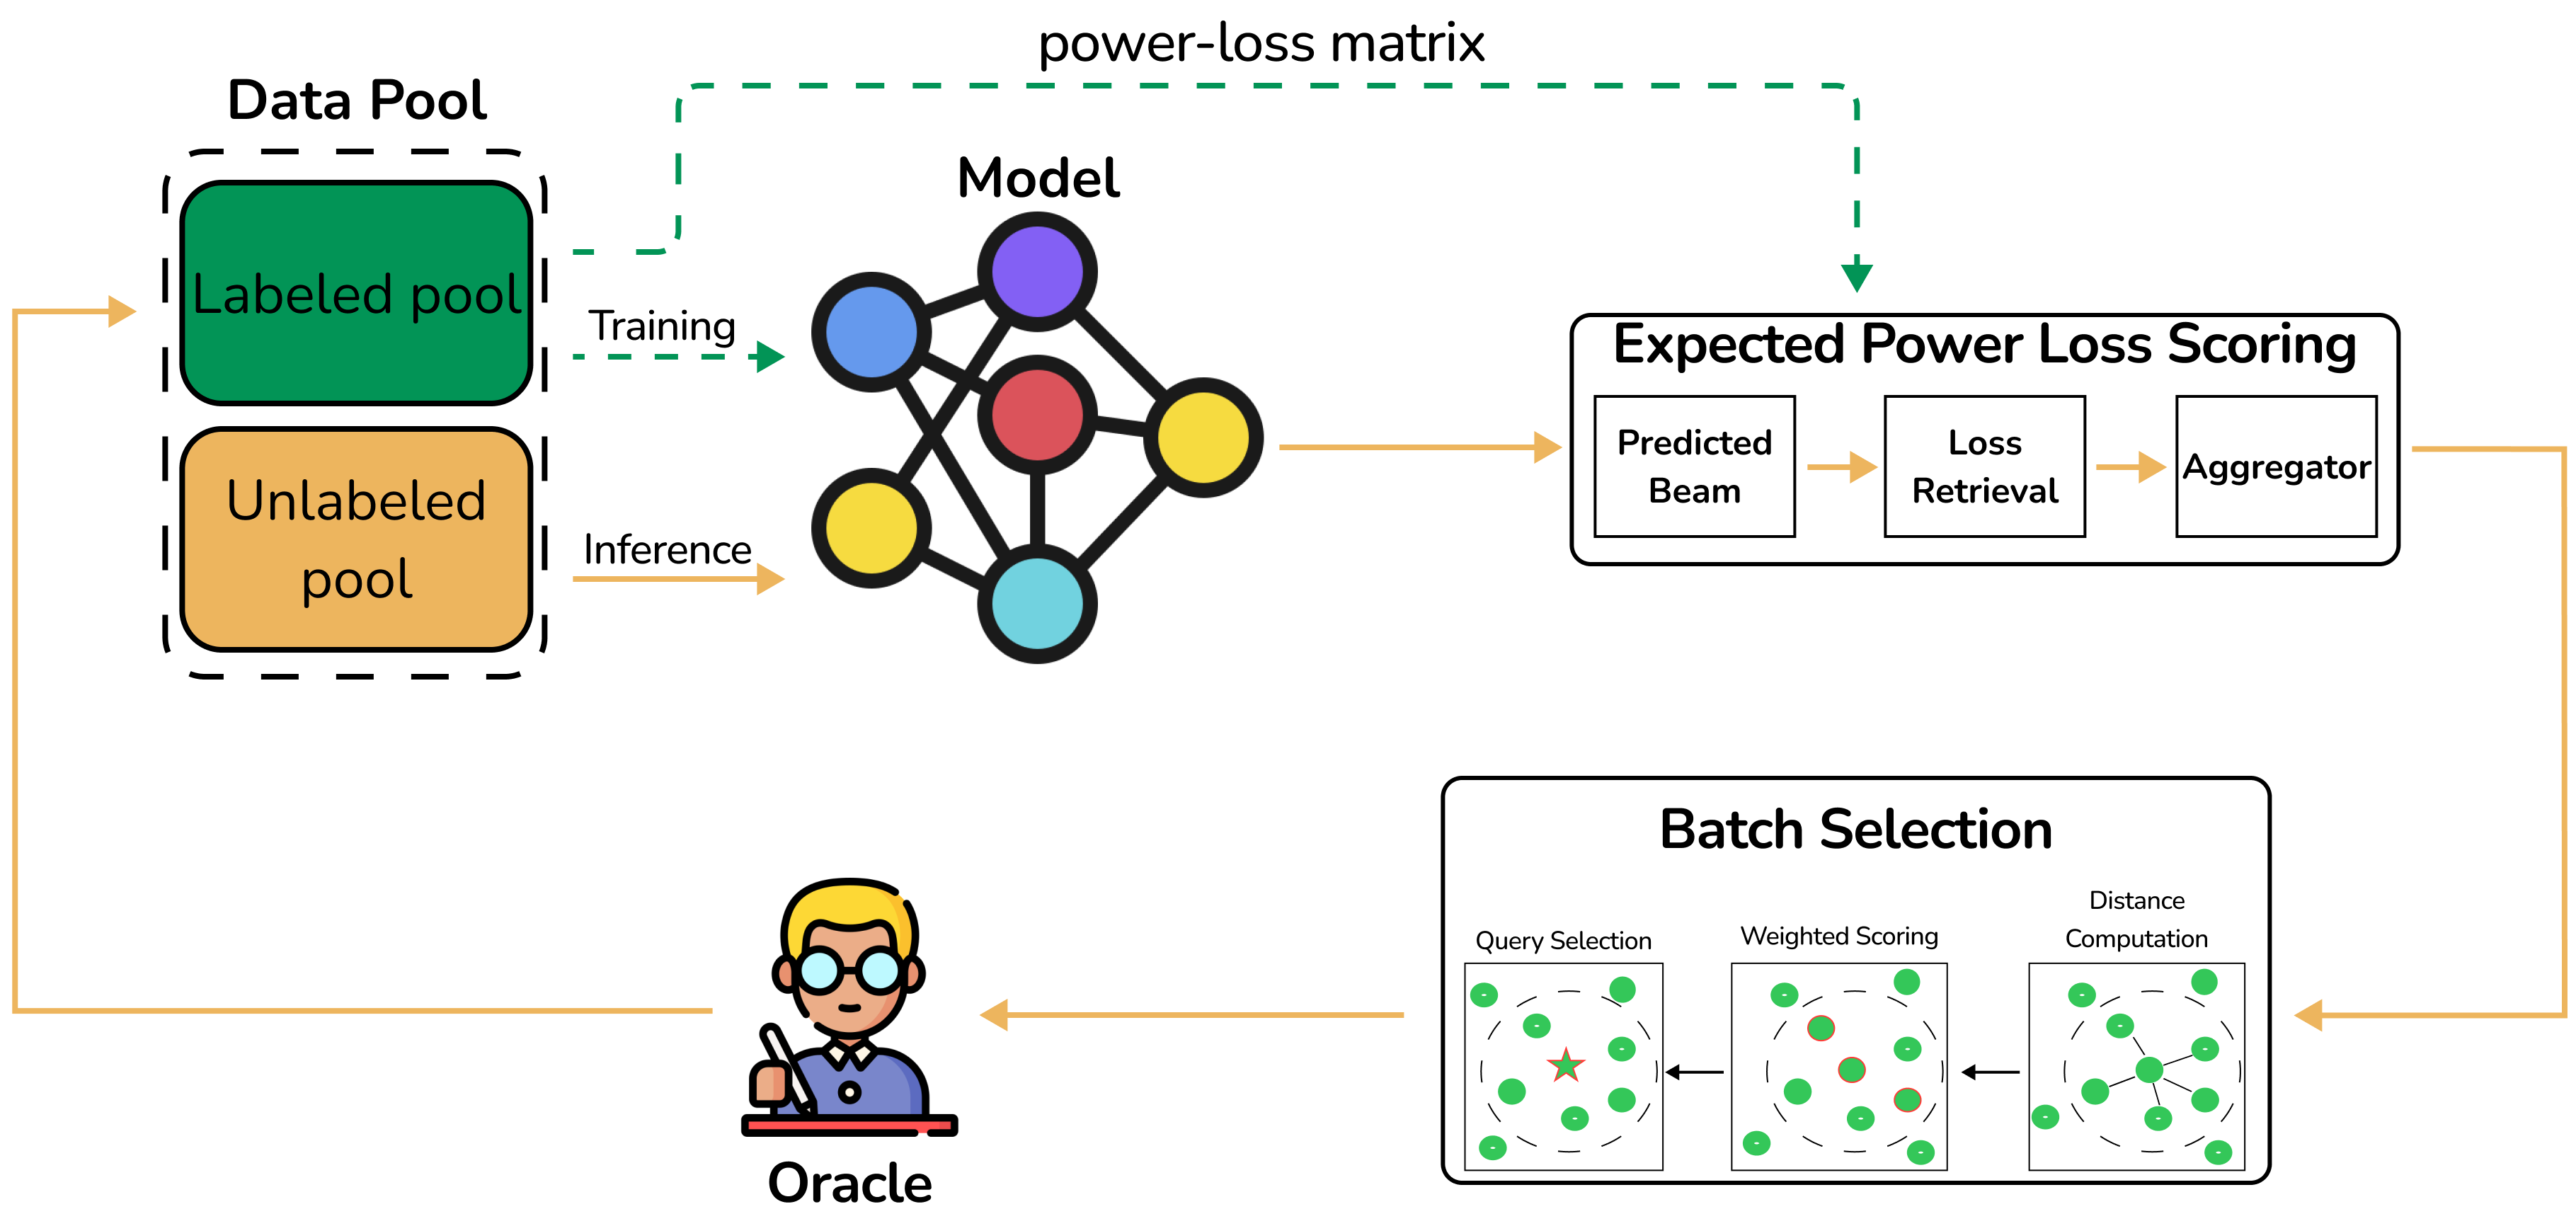
\includegraphics[width=\linewidth]{PAAL}
  \caption{Overview of the PAAL framework. Measured beam powers are used to create soft labels for training and to score the unlabeled pool by expected power loss; a weighted k-center rule then selects a diverse batch. Exhaustive sweeps then label the selected samples.}
  \label{fig:framework}
\end{figure}

\subsection{Problem Formulation}
\label{sec:formulation}
We consider a fixed mmWave access point or base station that serves vehicles at 60~GHz. It uses a phased array with $K$ beams, while a camera or LiDAR observes the scene. The predictor $f_\theta$ maps sensor input $x$ to a probability $p_\theta(k \mid x)$ for each beam. At run time, it selects the beam $\hat a(x) = \arg\max_k p_\theta(k \mid x)$. For training, an exhaustive sweep measures the received power $\gamma_k(x)$ in dB for each beam $k$. The beam with the highest power, $y^{*}(x) = \arg\max_k \gamma_k(x)$, is recorded as the label. The power lost when the predictor selects a beam is

\begin{equation}
  \ell(x) = \gamma_{y^{*}(x)}(x) - \gamma_{\hat a(x)}(x) \ \ge 0 \quad \text{(dB)}.
  \label{eq:loss_db}
\end{equation}
A label therefore requires one exhaustive sweep and provides both the best beam $y^{*}(x)$ and the full power profile $\gamma(x) \in \mathbb{R}^{K}$. Given an unlabeled pool $\mathcal{U}$ and a budget of $B$ sweeps, AL seeks a labeled subset that maximizes test accuracy:

\begin{equation}
  \max_{\mathcal{L} \subset \mathcal{U}} \ \mathrm{Acc}\big(f_{\theta(\mathcal{L})}\big) \quad \text{s.t.} \quad |\mathcal{L}| \le B.
  \label{eq:al}
\end{equation}
Here, $\theta(\mathcal{L})$ is obtained by training the model from scratch on the labeled set $\mathcal{L}$. Following~\cite{soltani2024learning}, we solve this problem in rounds. The current model scores the unlabeled pool, the oracle labels a batch of $b$ samples, and the model is retrained on the expanded labeled set. Equivalently, for a fixed target accuracy, AL aims to minimize the number of required sweeps.

\subsection{Expected Power Loss Scoring}
At each round, the model processes every sample $x$ in the unlabeled pool $\mathcal{U}$ and returns its beam probabilities $p(\cdot \mid x)$ and its penultimate-layer embedding $h(x)$. PAAL uses the labeled pool $\mathcal{L}$ to estimate the power lost for each pair of the true best beam and the selected beam. For beams $k$ and $a$, the average loss is

\begin{equation}
  D(k,a) = \frac{1}{|\mathcal{L}_k|} \sum_{x \in \mathcal{L}_k} \big(\gamma_k(x) - \gamma_a(x)\big),
  \qquad \mathcal{L}_k = \{x \in \mathcal{L} : y^{*}(x) = k\}.
  \label{eq:D}
\end{equation}
If a beam has no labeled examples, its row in $D$ is set to the mean of the observed rows. The matrix is updated after every round. To score an unlabeled sample, PAAL first takes the beam $\hat a(x)$ that the model would select. It then reads from $D$ the loss for that beam under each possible best beam and weights those losses by the model's predicted probabilities:

\begin{equation}
  \mathrm{EPL}(x) = \sum_{k=1}^{K} p(k \mid x)\, D\big(k, \hat a(x)\big).
  \label{eq:epl}
\end{equation}
The result is the sample's expected power loss (EPL), measured in dB. Unlike entropy, EPL can remain low when the model is uncertain between beams with similar power, because choosing either beam causes little loss.

\subsection{Batch and Query Selection}
Selecting only the samples with the highest EPL could produce a batch of similar, consecutive frames. PAAL instead builds the batch $\mathcal{S}$ one sample at a time. For each unlabeled sample, it measures the squared distance between its embedding and the closest embedding in the labeled set or the current batch:

\begin{equation}
  d(x) = \min_{x' \in \mathcal{L} \cup \mathcal{S}} \big\| h(x) - h(x') \big\|^{2}.
  \label{eq:dist}
\end{equation}
At each step, PAAL multiplies this distance by the sample's EPL and selects the sample with the largest product:

\begin{equation}
  x^{\star} = \arg\max_{x \in \mathcal{U} \setminus \mathcal{S}} \ \mathrm{EPL}(x) \cdot d(x).
  \label{eq:kcenter}
\end{equation}
After each choice, the distances are updated using the newly selected sample. Selection continues until the batch contains $b$ samples. This rule favors samples with high expected loss while covering different parts of the embedding space. For embeddings of dimension $m$, the selection step costs $O(b\,|\mathcal{U}|\,m)$, the same order as Core-set~\cite{sener2018coreset}.

The oracle performs an exhaustive sweep for every selected sample and returns its best beam and full power profile. These samples are moved from $\mathcal{U}$ to $\mathcal{L}$, and the model is retrained from scratch. PAAL converts each power profile into a soft target using temperature $T$ in dB. It then trains the model with a weighted sum of the hard-label and soft-label cross-entropy losses:

\begin{equation}
  q_k(x) = \frac{\exp\big(\gamma_k(x)/T\big)}{\sum_{j=1}^{K} \exp\big(\gamma_j(x)/T\big)},
  \qquad
  \mathcal{L}_{\text{train}} = (1-w)\,\mathrm{CE}\big(y^{*}, p\big) + w\,\mathrm{CE}\big(q, p\big).
  \label{eq:train}
\end{equation}
Here, $\mathrm{CE}$ is cross-entropy. Such soft targets are also used in knowledge distillation, where they convey how similar the classes are~\cite{hinton2015distilling}; here, they are obtained directly from the measured powers rather than from a teacher network. Beams whose power is close to the maximum receive nonzero target probability, so the model can learn that several beams may be suitable. The model is retrained after each round until the sweep budget $B$ is used, as shown in Algorithm~\ref{alg:paal}.

\begin{algorithm}[!t]
  \caption{Power-Aware Active Learning (PAAL)}
  \label{alg:paal}
  \begin{algorithmic}[1]
    \Require Unlabeled pool $\mathcal{U}$, initial size $n_0$, batch size $b$, budget $B$, soft-label parameters $T$ and $w$
    \Ensure Trained beam predictor $f_\theta$
    \State Draw $n_0$ samples from $\mathcal{U}$ at random, query the oracle for their $y^{*}(x)$ and $\gamma(x)$, and move them to $\mathcal{L}$
    \State Train $f_\theta$ from scratch on $\mathcal{L}$ with the loss \eqref{eq:train}
    \While{$|\mathcal{L}| < B$}
    \State Compute the power-loss matrix $D$ from $\mathcal{L}$ with \eqref{eq:D}
    \For{each $x \in \mathcal{U}$}
    \State Obtain $p(\cdot \mid x)$ and $h(x)$ from $f_\theta$, and set $\hat a(x) \gets \arg\max_a p(a \mid x)$
    \State Compute $\mathrm{EPL}(x)$ with \eqref{eq:epl} and $d(x)$ with \eqref{eq:dist}, where $\mathcal{S} = \emptyset$
    \EndFor
    \State $\mathcal{S} \gets \emptyset$
    \While{$|\mathcal{S}| < b$}
    \State $x^{\star} \gets \arg\max_{x \in \mathcal{U} \setminus \mathcal{S}} \mathrm{EPL}(x) \cdot d(x)$
    \State $\mathcal{S} \gets \mathcal{S} \cup \{x^{\star}\}$
    \State $d(x) \gets \min\big\{d(x), \|h(x) - h(x^{\star})\|^{2}\big\}$ for all $x \in \mathcal{U}$
    \EndWhile
    \State Query the oracle for $y^{*}(x)$ and $\gamma(x)$ of every $x \in \mathcal{S}$
    \State $\mathcal{L} \gets \mathcal{L} \cup \mathcal{S}$, \ $\mathcal{U} \gets \mathcal{U} \setminus \mathcal{S}$
    \State Train $f_\theta$ from scratch on $\mathcal{L}$ with the loss \eqref{eq:train}
    \EndWhile
    \State \Return $f_\theta$
  \end{algorithmic}
\end{algorithm}

%% ======================================================================
\section{Experimental Results and Discussion}
\label{sec:eval}

We test PAAL on both datasets and both modalities. The experiments measure how much AL reduces the number of required sweeps, how soft labels affect accuracy, and how PAAL compares with the baselines. We also study the effect of each PAAL component and discuss the results.

\subsection{Experimental Setup}
\subsubsection{Datasets}
We use two public datasets that match the system in Section~\ref{sec:formulation}. They differ in codebook size, sensor location, and power coverage. Each sample includes a camera image or a LiDAR scan, the best beam $y^{*}$, and the power profile $\gamma$ from the sweep.

\textbf{FLASH}~\cite{salehi2022flash} was collected as an automated car drove past a roadside mmWave radio. Both radio devices are TP-Link Talon AD7200 routers that use IEEE 802.11ad and a codebook of $K=34$ sectors. The GPS receiver, camera, and LiDAR are mounted on the car. The processed dataset contains 31\,363 synchronized samples. The sector labels are highly imbalanced: the smallest sector has 10 samples, while a few sectors occur in most samples. Each sweep measures about half of the 34 sectors. We set the unmeasured sectors to a noise floor equal to the 1st percentile of the measured power, so FLASH has an incomplete power profile. The camera input is an RGB image resized by bilinear interpolation to $3 \times 90 \times 160$ pixels, following~\cite{soltani2024learning}. The released LiDAR input is a binary $20 \times 20 \times 20$ occupancy grid; a voxel is set to one if it contains a LiDAR return.

\textbf{DeepSense~6G, scenario 32}~\cite{alkhateeb2023deepsense} was recorded during the day at a base station that serves passing vehicles. The station uses a 60~GHz phased array with a codebook of 64 beams. The camera and LiDAR are also mounted at the base station. The dataset contains 3\,235 samples, and 61 of the 64 beams appear as the best beam, with between 2 and 431 samples per beam. Each sample includes the measured power of all 64 beams; we convert these values to dB, so the power profile is complete. The camera image is resized to $3 \times 270 \times 480$ pixels, three times the FLASH resolution in each dimension. We keep this higher resolution because the camera is mounted at the base station and views passing vehicles from a distance, so each vehicle covers only a small part of the frame. All methods use the same resolution. DeepSense provides raw point clouds. We convert each scan to a binary $20 \times 20 \times 20$ occupancy grid using a box centered on the sensor. The box extends $\pm 20$~m horizontally and from $-3$ to $5$~m vertically, and it retains about 82\% of the points.

\subsubsection{Baselines}
We compare PAAL with five pool-based active learning methods. Random sampling selects samples uniformly from the unlabeled pool and serves as the reference for training on a random subset. Least confidence selects samples for which the model's highest predicted class probability is lowest; this method is called confidence sampling in~\cite{soltani2024learning}. Entropy sampling selects samples with the highest predictive entropy~\cite{settles2009survey}. GALAXY uses a search on a graph for class boundaries and was designed for imbalanced data~\cite{zhang2022galaxy}. Core-set uses a k-center strategy to select samples that cover the model's embedding space~\cite{sener2018coreset}.

Each baseline is evaluated with both hard and power-aware soft labels. With hard labels, the target is the index of the beam with the highest measured power, and the model is trained with standard cross-entropy, following~\cite{soltani2024learning}. With soft labels, every baseline uses the same target and loss as PAAL in~\eqref{eq:train}. This paired evaluation separates the effect of the training target from the effect of the acquisition method.

\subsubsection{Implementation Details}
We train a separate model for each modality and do not use GPS data. Each LiDAR input is a binary occupancy grid with one channel and dimensions $20 \times 20 \times 20$. The LiDAR model is a residual 3-D CNN with three convolution stages of 32, 64, and 128 channels, followed by global average pooling and a linear classifier. The pooled 128-dimensional feature is used as the embedding $h(x)$. Camera inputs are RGB images resized to $3 \times 90 \times 160$ for FLASH and $3 \times 270 \times 480$ for DeepSense~6G. We use the torchvision ResNet18~\cite{he2016resnet}, as in~\cite{soltani2024learning}, initialized at random and with a classifier that returns $K$ beam scores. Its pooled 512-dimensional feature is used as $h(x)$. We scale pixel values to $[0,1]$ and apply random color jitter to camera images during training.

All models use Adam with a learning rate of $10^{-3}$ and a batch size of 64. We train for at most 60 epochs and stop if the training loss improves by less than $10^{-3}$ for five consecutive epochs, with a minimum of 10 epochs. We retrain each model from scratch after every AL round. PAAL uses a soft-label temperature of $T=1$~dB and a hard/soft target weight of $w=0.5$. Table~\ref{tab:params} lists the remaining model, training, software, and hardware settings.

\subsubsection{Evaluation Protocol}

We follow the evaluation protocol in~\cite{soltani2024learning}. We shuffle each dataset and create a test set with 10 samples per beam. If a beam has fewer than 20 samples, we use half of them instead. This gives FLASH 335 test samples and a pool of 31\,028 samples. DeepSense has 520 test samples and a pool of 2\,715 samples. The pool remains imbalanced, as in the original data. We label an initial 5\% of the pool at random, then query another 5\% in each round, up to 50\%. Unlike~\cite{soltani2024learning}, we stop at 50\% because the methods differ most when the label budget is small. We retrain each network from scratch in every round. We run three seeds, each with its own data split. Within each seed, all methods share the same test set and initial labeled set.

\begin{table}[!t]
  \renewcommand{\arraystretch}{1.2}
  \caption{Dataset and training settings. The table lists the data, model, training, software, and hardware settings for both datasets.}
  \label{tab:params}
  \centering
  \footnotesize
  \begin{tabular}{|l|>{\raggedright\arraybackslash}p{0.33\linewidth}|>{\raggedright\arraybackslash}p{0.33\linewidth}|}
    \hline
    \textbf{Parameter} & \textbf{FLASH} & \textbf{DeepSense 6G (scenario 32)} \\
    \hline
    Link & 60~GHz IEEE 802.11ad, $K = 34$ sectors & 60~GHz phased array, $K = 64$ beams \\
    Samples & 31\,363 (pool 31\,028, test 335) & 3\,235 (pool 2\,715, test 520) \\
    Power profile & About half of the sectors measured per sweep & All 64 beams measured \\
    Camera input & RGB, $3 \times 90 \times 160$ & RGB, $3 \times 270 \times 480$ \\
    LiDAR input & $20^3$ occupancy grid released with the dataset & $20^3$ occupancy grid voxelized from point clouds \\
    AL budget & Initial set and batch of 1\,551 (5\%); up to 15\,510 (50\%) & Initial set and batch of 136 (5\%); up to 1\,360 (50\%) \\
    Full pool accuracy (top-1 / top-5) & LiDAR 0.807 / 0.970; camera 0.778 / 0.971 & LiDAR 0.142 / 0.503; camera 0.299 / 0.703 \\
    \hline
    LiDAR model & \multicolumn{2}{>{\raggedright\arraybackslash}p{0.68\linewidth}|}{Residual 3-D CNN (3 conv stages, 32/64/128 channels) on $20 \times 20 \times 20$ occupancy grids} \\
    Camera model & \multicolumn{2}{>{\raggedright\arraybackslash}p{0.68\linewidth}|}{ResNet18 \cite{he2016resnet}, random initialization, data augmentation} \\
    Training & \multicolumn{2}{>{\raggedright\arraybackslash}p{0.68\linewidth}|}{Adam, learning rate $10^{-3}$, batch size 64, at most 60 epochs; early stop when the training loss improves by less than $10^{-3}$ for 5 epochs (minimum 10 epochs); retrained from scratch every round} \\
    Soft labels & \multicolumn{2}{l|}{$T = 1$~dB, $w = 0.5$} \\
    Runs & \multicolumn{2}{l|}{Seeds 1, 10, 100 (each with its own split); 10 AL rounds per run} \\
    Software & \multicolumn{2}{>{\raggedright\arraybackslash}p{0.68\linewidth}|}{Python 3.12, PyTorch, torchvision} \\
    Hardware & \multicolumn{2}{l|}{NVIDIA GeForce RTX 4090 GPU} \\
    \hline
  \end{tabular}
\end{table}

\subsubsection{Experiment Plan and Metrics}
We run three experiments for each dataset and modality. First, we train all five baselines with hard labels to reproduce the setting in~\cite{soltani2024learning}. Second, we train the same baselines with soft labels to measure the effect of the training target. Third, we compare PAAL with the soft-label baselines and, on FLASH, with the PAAL ablations to measure the effect of the query method.

After each round, we measure top-1 and top-5 accuracy on the test set. We summarize each learning curve with its AUC, defined here as the mean accuracy over the 10 budget points and equal to the normalized area under the accuracy--budget curve. We also report the number of sweeps needed for the mean curve across seeds to reach each target accuracy, measured in steps of one batch, and the savings compared with random sampling. We do not smooth the curves, unlike~\cite{soltani2024learning}. On DeepSense, top-1 accuracy remains low even when the full pool is labeled: 61 narrow beams appear in the data, and nearby beams often have similar power. We therefore also report top-5 accuracy, which reflects selecting five candidate beams.

\subsection{Performance Comparison}
\emph{Hard labels on FLASH:} Figure~\ref{fig:hard} shows the hard-label baselines on FLASH. All uncertainty methods outperform random sampling for both modalities. For LiDAR, entropy and least confidence have the highest AUC values, 0.483 and 0.479. Both reach 60\% top-1 accuracy after 12\,408 labels, 20\% fewer than random sampling, which needs 15\,510. For camera data, Core-set has the highest AUC (0.546) and reaches 60\% accuracy with 9\,306 labels, 40\% fewer than random sampling. The best method therefore depends on the modality: Core-set performs best on camera data but worst on LiDAR, where its AUC (0.404) is below that of random sampling. GALAXY is not the best method for either modality in this budget range. No hard-label method reaches 70\% top-1 accuracy on LiDAR with at most 50\% of the pool.

\begin{figure}[!t]
  \centering
  \subfloat[LiDAR]{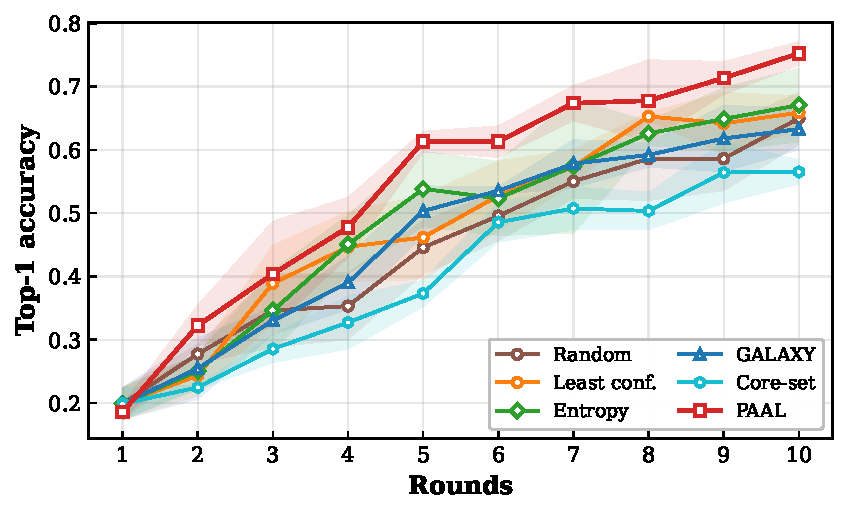
\includegraphics[width=0.48\linewidth]{flash_lidar_a_vs_hard_accuracy_vs_rounds}%
  \label{fig:hard_lidar}}
  \hfil
  \subfloat[Camera]{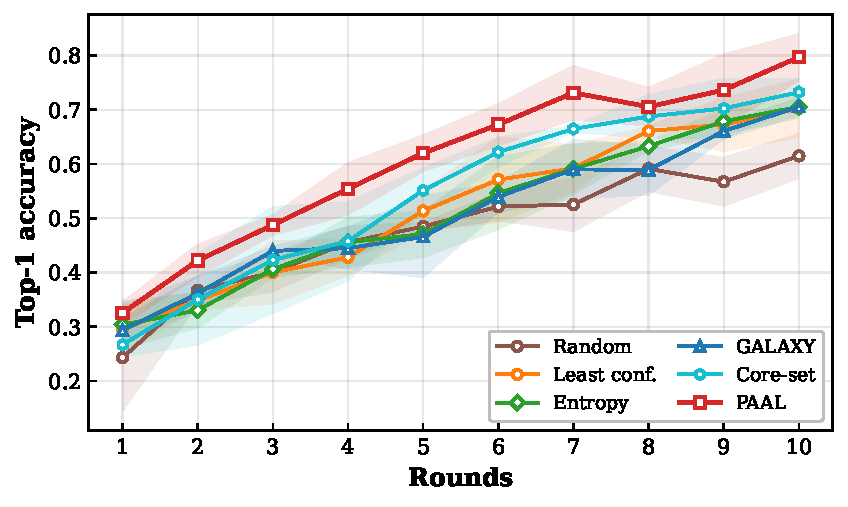
\includegraphics[width=0.48\linewidth]{flash_image_a_vs_hard_accuracy_vs_rounds}%
  \label{fig:hard_image}}
  \caption{Top-1 accuracy on FLASH over the active learning rounds. The baselines use hard labels, and PAAL, trained with soft labels, is included for comparison. The initial labeled set contains 5\% of the pool, and each later round adds 5\% (1\,551 samples). Shaded bands show $\pm 1$ standard deviation across three runs.}
  \label{fig:hard}
\end{figure}

We next test the methods on DeepSense~6G, which has a different site, codebook, and sensor setup. Table~\ref{tab:ds} and Fig.~\ref{fig:ds} show the results. Accuracy is lower than on FLASH. DeepSense has a larger codebook, about one tenth as many samples, and only 136 labels in the first round across 61 beams, or about two samples per beam. LiDAR performs poorly: even with the full pool, its top-1 accuracy is 0.142 and its top-5 accuracy is 0.503. We therefore focus on top-5 accuracy for LiDAR, since top-1 accuracy stays below 0.15 even with the full pool.

On DeepSense, uncertainty methods also outperform random sampling, but the best method again depends on the modality. Least confidence has a top-5 AUC of 0.227 on LiDAR, compared with 0.193 for random sampling. For camera data, Core-set has a top-5 AUC of 0.580, compared with 0.481 for random sampling. GALAXY is not the best method for either modality.

\emph{Effect of soft labels:} On FLASH, Fig.~\ref{fig:hard} and Fig.~\ref{fig:soft} compare hard-label and soft-label training. Soft labels raise the AUC of every method by 2.5--12.9 points on LiDAR and 1.6--4.6 points on camera data. The result holds in 35 of 36 combinations of method, run, and modality. The only decrease is 0.4 points for least confidence on camera data in one run. Core-set on LiDAR gains the most, 12.9 points, and moves from the weakest hard-label method to the strongest soft-label baseline. These gains require no extra sweeps because the oracle already returns the power profile $\gamma$. Comparing PAAL with hard-label baselines would mix the effect of the training target with the effect of sample selection, so the remaining comparisons use soft-label baselines.

On DeepSense~6G, soft labels raise the top-1 AUC of every method by 0.8--3.8 points on LiDAR and 2.3--4.6 points on camera data. The top-5 AUC rises by 4.6--11.8 points on LiDAR and 13.3--15.7 points on camera data. The top-1 AUC improves in 35 of 36 method and run combinations; the only decrease is 0.9 points for entropy on LiDAR in one run. DeepSense measures all 64 beams, so this result shows that the gain on FLASH does not depend on filling missing sector measurements with a noise floor. On camera data, soft-label methods exceed the top-5 accuracy of the model trained on the full pool with hard labels (0.703) after using only 15--35\% of the pool; Fig.~\ref{fig:ds_image} shows this result.

\subsection{Effectiveness of Power-Aware Acquisition}
\emph{FLASH:} Table~\ref{tab:s3} and Fig.~\ref{fig:soft} compare PAAL with the soft-label baselines. On camera data, PAAL has the highest AUC (0.605, versus 0.589 for Core-set), the highest top-5 AUC, and a small variation across runs ($\pm 0.010$). It reaches 60\% and 70\% top-1 accuracy with 7\,755 and 10\,857 labels, the same counts as Core-set, and reaches 0.797 accuracy after 50\% of the pool is labeled. This is slightly above the 0.778 result from training on the full pool. However, the difference is within the variation across runs on a test set of 335 samples, so we do not conclude that PAAL is better than full supervision. On LiDAR, PAAL exceeds the best soft-label baseline by 1.0 point (0.543 versus 0.533) and is the first method to reach 60\% top-1 accuracy, with 7\,755 labels. The EPL-only ablation has a higher AUC on LiDAR (0.556) and the lowest variation across runs ($\pm 0.003$).

\begin{table}[!t]
  \renewcommand{\arraystretch}{1.2}
  \caption{Results on FLASH with soft labels. Values are means over three runs, with standard deviations shown where available. The table reports AUC, top-5 AUC, top-1 accuracy at 50\% of the pool, and label counts needed to reach 60\% ($N_{60}$) and 70\% ($N_{70}$) top-1 accuracy.}
  \label{tab:s3}
  \centering
  \footnotesize
  \setlength{\tabcolsep}{4pt}
  \begin{tabular}{|l|c|c|c|c|c||c|c|c|c|c|}
    \hline
    \multirow{2}{*}{\textbf{Methods (soft labels)}} & \multicolumn{5}{c||}{\textbf{LiDAR}} & \multicolumn{5}{c|}{\textbf{Camera}} \\
    \cline{2-11}
    & AUC & AUC top-5 & @50\% & $N_{60}$ & $N_{70}$ & AUC & AUC top-5 & @50\% & $N_{60}$ & $N_{70}$ \\
    \hline
    Random      & 0.485 $\pm$ 0.004 & 0.756 & 0.660 & 12\,408 & -- & 0.520 $\pm$ 0.024 & 0.773 & 0.645 & 13\,959 & -- \\
    Least conf. & 0.510 $\pm$ 0.017 & 0.789 & 0.715 & 10\,857 & 15\,510 & 0.535 $\pm$ 0.042 & 0.782 & 0.691 & 9\,306 & -- \\
    Entropy     & 0.512 $\pm$ 0.021 & 0.784 & 0.723 & 10\,857 & 15\,510 & 0.528 $\pm$ 0.008 & 0.791 & 0.691 & 12\,408 & -- \\
    GALAXY      & 0.488 $\pm$ 0.013 & 0.769 & 0.725 & 12\,408 & 13\,959 & 0.555 $\pm$ 0.016 & 0.792 & 0.739 & 10\,857 & 15\,510 \\
    Core-set    & 0.533 $\pm$ 0.011 & 0.796 & 0.723 & 10\,857 & 13\,959 & 0.589 $\pm$ 0.022 & 0.814 & 0.718 & \textbf{7\,755} & \textbf{10\,857} \\
    \hline
    \textbf{PAAL}      & \textbf{0.543 $\pm$ 0.013} & \textbf{0.804} & \textbf{0.752} & \textbf{7\,755} & 13\,959 & \textbf{0.605 $\pm$ 0.010} & \textbf{0.822} & \textbf{0.797} & \textbf{7\,755} & \textbf{10\,857} \\
    \hline
  \end{tabular}
\end{table}

\begin{figure}[!t]
  \centering
  \subfloat[LiDAR]{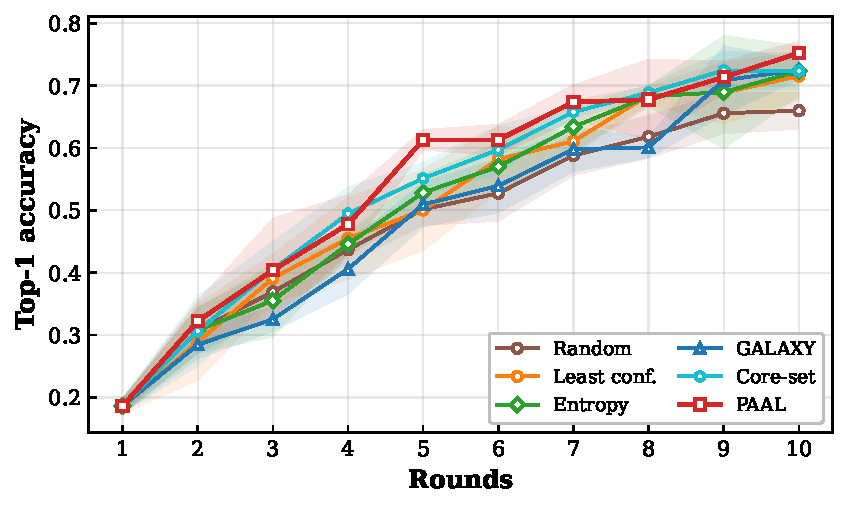
\includegraphics[width=0.48\linewidth]{flash_lidar_b_vs_soft_accuracy_vs_rounds}%
  \label{fig:soft_lidar}}
  \hfil
  \subfloat[Camera]{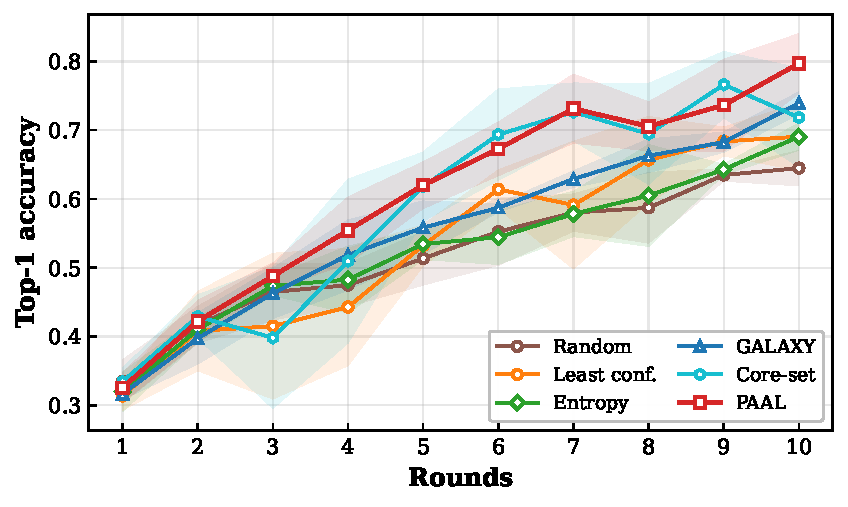
\includegraphics[width=0.48\linewidth]{flash_image_b_vs_soft_accuracy_vs_rounds}%
  \label{fig:soft_image}}
  \caption{Top-1 accuracy on FLASH over the active learning rounds with soft labels. All methods use soft labels; round and shading conventions are the same as in Fig.~\ref{fig:hard}.}
  \label{fig:soft}
\end{figure}

\emph{Variation across runs:} We compare PAAL with the strongest baseline in each run. Core-set with soft labels is the strongest competitor in all six runs. PAAL wins two of the three runs for each modality, by 0.8--3.4 points, and loses the run with seed 1 on both modalities, by 1.1 points on LiDAR and 0.6 points on camera data. With only three runs, the mean gain of 1.0 point on LiDAR is smaller than the variation between runs and is not conclusive. The 1.6-point gain on camera data is more consistent.

\emph{DeepSense~6G:} The best method depends on the modality. On LiDAR, PAAL has the highest top-1 and top-5 AUC values, 0.089 and 0.332. It exceeds the best other method in top-5 AUC in all three runs, by 0.8, 1.8, and 1.3 points, and in top-1 AUC in two runs. On camera data, Core-set with soft labels performs best, with top-1 and top-5 AUC values of 0.282 and 0.734. It exceeds PAAL in every run by 0.6--2.1 points in top-1 AUC and 0.9--1.6 points in top-5 AUC.

\begin{table}[!t]
  \renewcommand{\arraystretch}{1.2}
  \caption{Results on DeepSense~6G. Values are means over three runs, with standard deviations shown where available. Top-5@50\% denotes top-5 accuracy after labeling 50\% of the pool.}
  \label{tab:ds}
  \centering
  \footnotesize
  \begin{tabular}{|l|l|c|c|c||c|c|c|}
    \hline
    \multirow{2}{*}{\textbf{Labels}} & \multirow{2}{*}{\textbf{Methods}} & \multicolumn{3}{c||}{\textbf{LiDAR}} & \multicolumn{3}{c|}{\textbf{Camera}} \\
    \cline{3-8}
    & & AUC top-1 & AUC top-5 & Top-5@50\% & AUC top-1 & AUC top-5 & Top-5@50\% \\
    \hline
    \multirow{5}{*}{Hard}
    & Random      & 0.048 & 0.193 $\pm$ 0.009 & 0.243 & 0.195 & 0.481 $\pm$ 0.002 & 0.663 \\
    & Least conf. & 0.056 & 0.227 $\pm$ 0.008 & 0.403 & 0.222 & 0.540 $\pm$ 0.016 & 0.706 \\
    & Entropy     & 0.055 & 0.214 $\pm$ 0.023 & 0.299 & 0.216 & 0.539 $\pm$ 0.023 & 0.666 \\
    & GALAXY      & 0.042 & 0.176 $\pm$ 0.001 & 0.268 & 0.206 & 0.511 $\pm$ 0.039 & 0.661 \\
    & Core-set    & 0.040 & 0.179 $\pm$ 0.012 & 0.313 & 0.236 & 0.580 $\pm$ 0.007 & 0.699 \\
    \hline
    \multirow{6}{*}{Soft}
    & Random      & 0.056 & 0.239 $\pm$ 0.011 & 0.396 & 0.231 & 0.626 $\pm$ 0.014 & 0.800 \\
    & Least conf. & 0.068 & 0.274 $\pm$ 0.014 & 0.419 & 0.254 & 0.677 $\pm$ 0.006 & 0.832 \\
    & Entropy     & 0.072 & 0.280 $\pm$ 0.046 & 0.486 & 0.255 & 0.672 $\pm$ 0.025 & 0.828 \\
    & GALAXY      & 0.075 & 0.285 $\pm$ 0.011 & 0.431 & 0.244 & 0.668 $\pm$ 0.006 & 0.829 \\
    & Core-set    & 0.078 & 0.293 $\pm$ 0.029 & 0.429 & \textbf{0.282} & \textbf{0.734 $\pm$ 0.002} & \textbf{0.834} \\
    & \textbf{PAAL} & \textbf{0.089} & \textbf{0.332 $\pm$ 0.012} & \textbf{0.492} & 0.270 & 0.722 $\pm$ 0.004 & 0.826 \\
    \hline
  \end{tabular}
\end{table}

\begin{figure}[!t]
  \centering
  \subfloat[LiDAR]{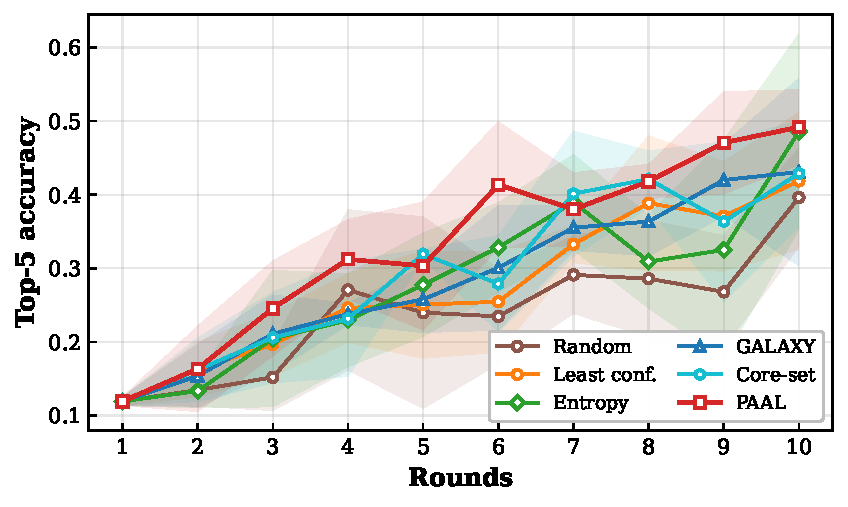
\includegraphics[width=0.48\linewidth]{deepsense_lidar_soft_top5_vs_rounds}%
  \label{fig:ds_lidar}}
  \hfil
  \subfloat[Camera]{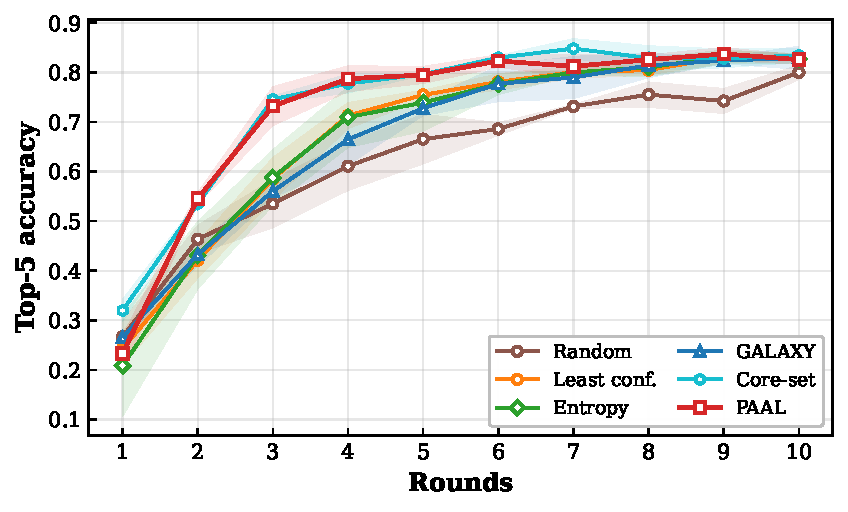
\includegraphics[width=0.48\linewidth]{deepsense_image_soft_top5_vs_rounds}%
  \label{fig:ds_image}}
  \caption{Top-5 accuracy on DeepSense~6G over the active learning rounds with soft labels. Each round adds 5\% of the pool (136 samples), and shaded bands show $\pm 1$ standard deviation across three runs.}
  \label{fig:ds}
\end{figure}

\subsection{Ablation Study}
We study the PAAL components on FLASH, where the methods differ most. Figure~\ref{fig:ablation} shows the result of removing one component at a time. Removing soft labels has the largest effect: AUC falls from 0.543 to 0.468 on LiDAR and from 0.605 to 0.563 on camera data. Removing the EPL weight gives Core-set with soft labels and lowers AUC by 1.0 point on LiDAR (to 0.533) and 1.6 points on camera data (to 0.589). Removing k-center leaves EPL-only ranking and has different effects on the two modalities. On camera data, AUC falls by 5.5 points to 0.550, and accuracy changes sharply between rounds (Fig.~\ref{fig:abl_image}). On LiDAR, AUC rises by 1.3 points to 0.556. Thus, soft labels and EPL improve both modalities, but the value of k-center depends on the modality. We expect k-center to help when embeddings separate samples well, as the ResNet18 camera embedding appears to do. We have not tested this explanation.

\begin{figure}[!t]
  \centering
  \subfloat[LiDAR]{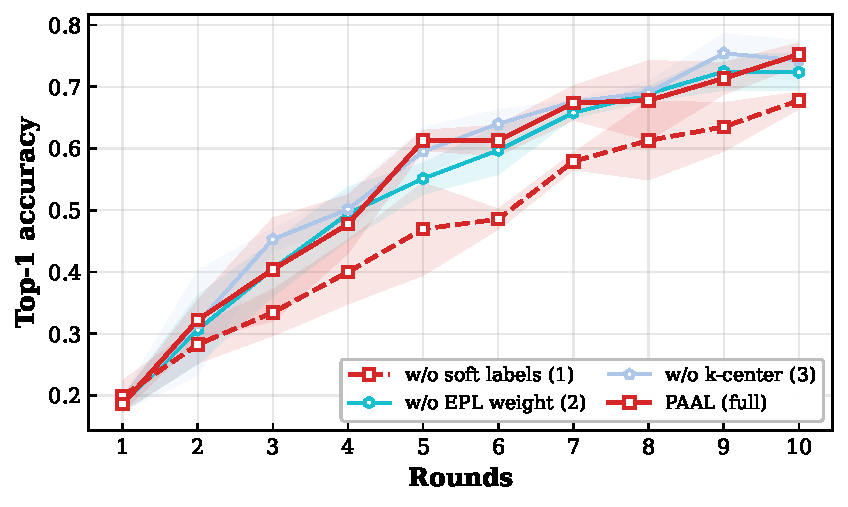
\includegraphics[width=0.48\linewidth]{flash_lidar_c_ablation_accuracy_vs_rounds}%
  \label{fig:abl_lidar}}
  \hfil
  \subfloat[Camera]{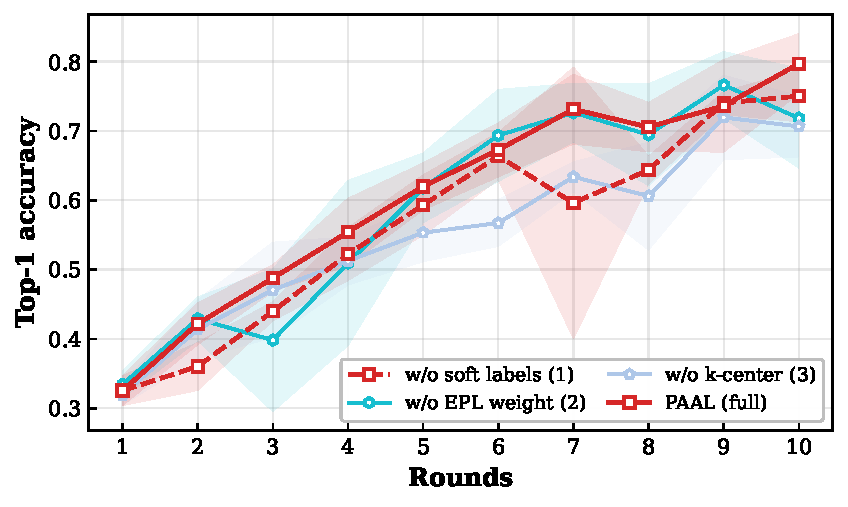
\includegraphics[width=0.48\linewidth]{flash_image_c_ablation_accuracy_vs_rounds}%
  \label{fig:abl_image}}
  \caption{Top-1 accuracy on FLASH for PAAL and its ablations. Each version removes one component; the dashed red line shows PAAL trained with hard labels, and shaded bands show $\pm 1$ standard deviation over three runs.}
  \label{fig:ablation}
\end{figure}

\subsection{Computational Cost}
All methods use the same backbone and add no trainable parameters. Training and inference costs are therefore the same across methods and depend on the backbone. The LiDAR network has 0.56~M parameters and needs 0.35~GFLOPs per sample. ResNet18 has 11.2~M parameters and needs 1.09~GFLOPs per FLASH sample and 9.56~GFLOPs per DeepSense sample. The methods differ only in the time needed to select a batch. Table~\ref{tab:cost} reports the selection time alone. We measured it on a CPU using the labels and sweeps in each dataset, with pools of at most 3\,000 samples, and averaged the results over AL rounds in three runs.

Random sampling and the uncertainty methods select a batch in less than 0.6~ms. GALAXY, Core-set, and PAAL take longer because they revisit the pool for each selected sample. GALAXY takes 132--230~ms per round. Core-set and PAAL take 47--82~ms with the 128-dimensional LiDAR embedding and 180--237~ms with the 512-dimensional ResNet18 embedding. PAAL adds at most 3.7~ms over Core-set. This added time comes from computing the power-loss matrix and EPL. Selection time grows in proportion to pool size and batch size. In the full FLASH runs, inference and selection with PAAL take on average 15~s per round with LiDAR and 24~s with camera data, compared with about 2~minutes to retrain the network. Its added computation is small compared with training and with the sweeps it can save.

\begin{table}[!t]
  \renewcommand{\arraystretch}{1.2}
  \caption{Batch selection time per round and backbone size. Selection times are means with standard deviations across three CPU runs; parameter counts and GFLOPs per sample are reported for each modality and dataset.}
  \label{tab:cost}
  \centering
  \footnotesize
  \begin{tabular}{|l|c|c||c|c|}
    \hline
    \multirow{2}{*}{\textbf{Methods}} & \multicolumn{2}{c||}{\textbf{FLASH}} & \multicolumn{2}{c|}{\textbf{DeepSense 6G}} \\
    \cline{2-5}
    & LiDAR & Camera & LiDAR & Camera \\
    \hline
    Random      & 0.09 $\pm$ 0.01 & 0.09 $\pm$ 0.01 & 0.09 $\pm$ 0.00 & 0.10 $\pm$ 0.02 \\
    Least conf. & 0.30 $\pm$ 0.02 & 0.26 $\pm$ 0.01 & 0.41 $\pm$ 0.08 & 0.33 $\pm$ 0.01 \\
    Entropy     & 0.48 $\pm$ 0.10 & 0.39 $\pm$ 0.01 & 0.56 $\pm$ 0.02 & 0.47 $\pm$ 0.02 \\
    GALAXY      & 139.08 $\pm$ 1.51 & 131.92 $\pm$ 1.86 & 229.90 $\pm$ 2.45 & 227.19 $\pm$ 2.07 \\
    Core-set    & 78.59 $\pm$ 7.13 & 235.69 $\pm$ 3.43 & 47.01 $\pm$ 1.86 & 180.16 $\pm$ 4.61 \\
    \textbf{PAAL} & 81.63 $\pm$ 5.21 & 237.49 $\pm$ 4.43 & 50.69 $\pm$ 1.63 & 180.19 $\pm$ 2.24 \\
    \hline
    Backbone parameters (M)  & 0.56 & 11.19 & 0.56 & 11.21 \\
    Backbone GFLOPs / sample & 0.35 & 1.09 & 0.35 & 9.56 \\
    \hline
  \end{tabular}
\end{table}

\subsection{Discussion}
\textbf{The power profile adds useful information:} The main finding is that soft labels from the power profile improve every method in every setting. This gain is larger than most differences between query methods, and it also appears on DeepSense, where the full profile is measured. The PAAL query rule gives an added gain in three of the four settings, but the best rule depends on the modality. Weighted k-center works best on FLASH camera data and DeepSense LiDAR. EPL-only ranking works best on FLASH LiDAR. Core-set with soft labels remains best on DeepSense camera data.

\textbf{Comparison with earlier work:} As in~\cite{soltani2024learning}, AL reduces the label cost on FLASH; we see the same result on DeepSense. However, with hard labels as in~\cite{soltani2024learning}, GALAXY does not outperform confidence sampling in our experiments. Several setup differences may explain this: we stop at 50\% of the pool, use batches of 1\,551 rather than 204 samples, do not smooth the curves, and use a FLASH release whose smallest class has 10 rather than 20 samples. GALAXY still selects rare classes as intended. On FLASH LiDAR with hard labels, it queries 4.7 of the five training samples from the smallest class by the 50\% budget, compared with 3.3 for random sampling. In this budget range, greater class coverage does not lead to higher accuracy. Core-set's strong results on camera data are consistent with its original image classification tests~\cite{sener2018coreset}.

\textbf{Implications for network design:} The main cost of deploying a beam predictor at a new site is collecting labels through exhaustive sweeps. Our results show that soft labels and AL can reach target accuracy with half as many sweeps on FLASH, or fewer on DeepSense, than random sampling with hard labels. On FLASH, PAAL reaches 60\% top-1 accuracy with 7\,755 labels for both modalities, while random sampling needs 15\,510. On DeepSense, PAAL reaches 30\% top-5 accuracy on LiDAR and 70\% on camera data with 544 and 408 labels, or 20\% and 15\% of the pool. Random sampling with hard labels does not reach these targets within the 50\% budget. Soft labels provide much of the gain and are simple to use: they change only the training loss and reuse measurements from the existing sweep. The beam training procedure in 802.11ad or 5G NR does not need to change. The query method has a smaller effect, so it should be checked for each modality.

%% ======================================================================
\section{Conclusion}
\label{sec:conclusion}
This work studies how to reduce the number of exhaustive sweeps needed to train a beam predictor that uses sensor data. We show that each sweep measures the power of every beam, while standard AL methods use only the strongest beam's index. We propose PAAL, which uses the full power profile for training, scoring, and batch selection. We test PAAL and five baselines on FLASH and DeepSense~6G with camera and LiDAR modalities. Standard AL reduces labeling cost on both datasets. On FLASH, the best hard-label method reaches 60\% top-1 accuracy with 20--40\% fewer labels than random sampling, although the best method depends on the modality. Soft labels improve every method in all four settings without extra sweeps. With soft labels, PAAL outperforms every baseline in three of the four settings and reaches its target accuracy with 15--25\% of the pool, while random sampling with hard labels needs at least 50\% or does not reach the target. Core-set with soft labels remains best on DeepSense camera data. These findings show the value of using the full power measurement, not only the index of the strongest beam.

\textbf{Limitations:} This study has several limitations. First, each setting uses three runs. PAAL loses one run on each FLASH modality and all runs on DeepSense camera data, so small differences between the leading methods are uncertain. Second, we split samples rather than full drive episodes. Consecutive frames from one drive may therefore appear in both the pool and test set, which may raise the measured accuracy. The test sets are also small, with 335 and 520 samples; one sample changes top-1 accuracy by 0.3 or 0.2 percentage points. Third, FLASH contains power measurements for only about half of its sectors. DeepSense has complete profiles and confirms the gain from soft labels, but it is about ten times smaller than FLASH. Fourth, LiDAR provides limited information on DeepSense with our $20^3$ voxel grid; its accuracy on the full data pool is 0.142. Finally, we test only five baselines, keep $T$ and $w$ fixed, and report classification accuracy rather than the power loss in~\eqref{eq:loss_db}, which is a more direct measure of link quality.

\textbf{Future work:} Future work will use five runs and splits that keep each drive episode entirely in either the pool or the test set. We will also evaluate predictors by power loss and achievable rate, not accuracy alone. Further work can compare PAAL with methods such as BADGE, BAIT, TypiClust, and ProbCover, and test how its results change with $T$ and $w$. Since no query rule wins in every setting, a method that chooses between EPL ranking, weighted k-center, and standard k-center based on the data may be useful. A finer or learned LiDAR representation may also improve DeepSense results and change the ranking of the methods.

\bibliographystyle{IEEEtran}
\bibliography{references}
\end{document}
